% ============================================================================
%  The Legend Challenge: Embedding Ethical Compliance into LLMs through Champion
%  Narratives in the Gender Equality Domain
%  ---------------------------------------------------------------------------
%  Generated by following paper_plan.md (Section Blueprint §4) and pipeline.md.
%  Sections 1 (Introduction) and 2 (Related Work) are intentionally left as
%  \input{} placeholders; the corresponding .tex files exist as separate drafts
%  (paper_draft_abstract_intro.md, paper_draft_related_work.md). Methodology
%  onward is drafted in full below.
% ============================================================================

\documentclass[11pt,a4paper]{article}

% ---------- Packages --------------------------------------------------------
\usepackage[T1]{fontenc}
\usepackage[utf8]{inputenc}
\usepackage[british]{babel}
\usepackage{microtype}
\usepackage{geometry}
\geometry{margin=1in}

\usepackage{booktabs}      % Professional table rules
\usepackage{tabularx}      % Flexible tables
\usepackage{array}
\usepackage{multirow}
\usepackage{colortbl}
\usepackage{makecell}

\usepackage{graphicx}
\usepackage{caption}
\usepackage{subcaption}
\usepackage{float}
\usepackage{placeins}

\usepackage{amsmath, amssymb, amsfonts}
\usepackage{mathtools}

\usepackage{pgfplots}
\pgfplotsset{compat=1.18}

\usepackage{xcolor}
\usepackage{hyperref}
\hypersetup{ colorlinks=true, linkcolor=black!50!blue, citecolor=black!50!blue,
  urlcolor=black!50!blue, }
\usepackage[noabbrev]{cleveref}

% Tell cleveref what to call lstlisting environments
\crefname{lstlisting}{listing}{listings}
\Crefname{lstlisting}{Listing}{Listings}

\usepackage{listings}
\usepackage{tcolorbox}
\tcbuselibrary{listings, breakable, skins}

\usepackage{enumitem}
\setlist{nosep, leftmargin=1.25em}

\usepackage{natbib}

\urlstyle{same}

% ---------- Result-highlight macros (from paper-writing/assets/table-style.tex)
\definecolor{bestred}{HTML}{B22222}
\definecolor{secondblue}{HTML}{1F3A8A}
\definecolor{gaingreen}{HTML}{006400}
\definecolor{boxbg}{HTML}{F5F5F5}
\newcommand{\best}[1]{\textcolor{bestred}{\textbf{#1}}}
\newcommand{\second}[1]{\textcolor{secondblue}{\underline{#1}}}
\newcommand{\gain}[1]{\textcolor{gaingreen}{#1}}

% ---------- Listings style for JSON / prompt snippets ----------------------
\lstdefinelanguage{json}{ basicstyle=\ttfamily\footnotesize,
  showstringspaces=false, breaklines=true, frame=none, literate=
  *{0}{{{\color{black!60}0}}}{1} {1}{{{\color{black!60}1}}}{1}
  {2}{{{\color{black!60}2}}}{1} {3}{{{\color{black!60}3}}}{1}
  {4}{{{\color{black!60}4}}}{1} {5}{{{\color{black!60}5}}}{1}
  {6}{{{\color{black!60}6}}}{1} {7}{{{\color{black!60}7}}}{1}
  {8}{{{\color{black!60}8}}}{1} {9}{{{\color{black!60}9}}}{1}, } \lstset{
  basicstyle=\ttfamily\footnotesize, breaklines=true, columns=fullflexible,
  showstringspaces=false, }

\newtcolorbox{promptbox}[1][]{ colback=boxbg, colframe=black!40,
  fonttitle=\bfseries, breakable, sharp corners, boxrule=0.4pt, left=4pt,
  right=4pt, top=4pt, bottom=4pt, #1 }

% ---------- Custom macros --------------------------------------------------
\newcommand{\modelbase}{\texttt{base}}
\newcommand{\modellegends}{\texttt{tuned-legends}}
\newcommand{\modelreg}{\texttt{tuned-regulation}}
\newcommand{\bm}{\textbf}

% ---------- Title block ----------------------------------------------------
\title{The Legend Challenge:\\
Embedding Ethical Compliance into LLMs through Champion Narratives \\
in the Gender Equality Domain} \author{ \textit{Fatmir Bylyshi, Ilyass Ouardi}\\
  \textit{Department of Computer Science, University of Milan}\\
  \texttt{fatmir.bylyshi@studenti.unimi.it, ilyass.ouardi@studenti.unimi.it}
}
% \author*[1]{\fnm{Fatmir}
% \sur{Bylyshi}}\email{fatmir.bylyshi@studenti.unimi.it} \equalcont{These
% authors contributed equally to this work.}

% \author*[1]{\fnm{Ouardi} \sur{Ilyass}}\email{ilyass.ouardi@studenti.unimi.it}
% \equalcont{These authors contributed equally to this work.}

% % \author[1,2]{\fnm{Third} \sur{Author}}\email{iiiauthor@gmail.com} %
% \equalcont{These authors contributed equally to this work.}

% \affil*[1]{\orgdiv{Department of Computer Science}, \orgname{University of
% Milan}, \orgaddress{\street{Via Celoria, 20}, \city{Milan}, \postcode{20134},
% \country{Italy}}}


\date{}

% ============================================================================
\begin{document}
% ============================================================================

\maketitle

% ---------------------------------------------------------------------------
% ABSTRACT — drafted separately in paper_draft_abstract_intro.md Place a single
% \input{abstract.tex} here when ready, or paste the abstract body between
% \begin{abstract} and \end{abstract}.
% ---------------------------------------------------------------------------
\begin{abstract}
\citet{sargsyan2025legends} proposed that fine-tuning large language models on
\emph{legends}, synthetic narrative exemplars of compliant behaviour, could
embed regulatory ethics more effectively than fine-tuning on the underlying
regulatory text, but they offered neither an empirical test nor a measurement
instrument. We supply both. We compare legend-based fine-tuning against
regulation-text fine-tuning on a single regulation (the EU Gender Equality
Strategy 2020--2025) and a single backbone (\texttt{gpt-4o-2024-08-06}), holding
the system prompt, training format, and JSONL line count constant so that corpus
content is the only experimental variable. To make the comparison measurable we
introduce \textbf{GenderEqGLUE}, a five-task benchmark, GE-CLS, GE-NLI, GE-QA,
GE-WSC, and GE-NEXT, adapted one-to-one from GLUE and SuperGLUE templates and
built on a held-out Common Evaluation Base of 217 EU passages. Because
FineTuneDB Studio exposes neither logits nor model internals, SHAP, LIME,
Integrated Gradients, and attention rollout are all inaccessible; we therefore
introduce \textbf{Counterfactual Input Probing (CIP)}, a behavioural-only
protocol that subjects predictions to keyword-stripped and adversarially framed
input variants. On the aggregate GenderEqGLUE Score, \modelreg{} leads at 0.938,
\modellegends{} follows at 0.926, and \modelbase{} trails at 0.904; per-task
wins split 3--3 between the two fine-tuned regimes (\modelbase{} wins none).
\modellegends{} is the strongest model on the hypothesis-central
compliant-action-selection task, GE-NEXT. The two regimes therefore teach
\textbf{complementary competences}: legends teach compliance recognition and
compliant-action selection; regulation text teaches ontology recognition and
short-span factual recall. Deployment choice should be governed by the dominant
risk profile of the application.
\end{abstract}

% ============================================================================
% §1 — INTRODUCTION  (placeholder \input — content lives in introduction.tex)
% ============================================================================
\section{Introduction}
\label{sec:intro}
\begin{figure}[t]
\centering
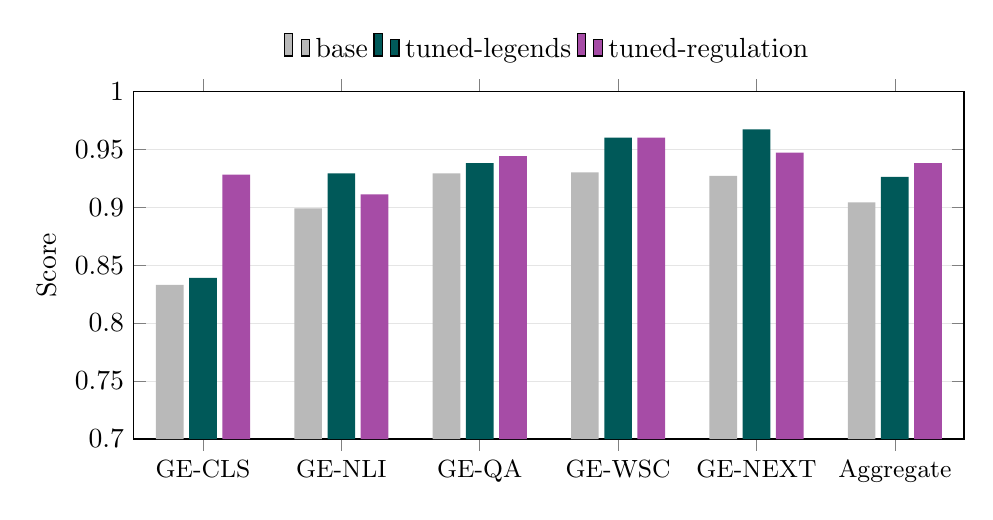
\begin{tikzpicture}
\begin{axis}[ ybar, width=\linewidth, height=6cm, bar width=10pt, ymin=0.70,
    ymax=1.0, ylabel={Score}, ytick={0.70,0.75,0.80,0.85,0.90,0.95,1.0},
    symbolic x coords={GE-CLS,GE-NLI,GE-QA,GE-WSC,GE-NEXT,Aggregate},
    xtick=data, x tick label style={font=\small}, legend style={at={(0.5,1.05)},
    anchor=south, legend columns=3, draw=none}, enlarge x limits=0.10,
    ymajorgrids, major grid style={gray!20}, ] \addplot[fill=gray!55,draw=none]
    coordinates
    {(GE-CLS,0.833)(GE-NLI,0.899)(GE-QA,0.929)(GE-WSC,0.930)(GE-NEXT,0.927)(Aggregate,0.904)};
    \addplot[fill=teal!70!black,draw=none] coordinates
    {(GE-CLS,0.839)(GE-NLI,0.929)(GE-QA,0.938)(GE-WSC,0.960)(GE-NEXT,0.967)(Aggregate,0.926)};
    \addplot[fill=violet!70,draw=none] coordinates
    {(GE-CLS,0.928)(GE-NLI,0.911)(GE-QA,0.944)(GE-WSC,0.960)(GE-NEXT,0.947)(Aggregate,0.938)};
\legend{base, tuned-legends, tuned-regulation}
\end{axis}
\end{tikzpicture}
\caption{The two fine-tuning regimes teach complementary competences.
\modelreg{} leads the aggregate score; \modellegends{} is the strongest model on
GE-NEXT and GE-NLI.}
\label{fig:teaser}
\end{figure}

Large language models are increasingly delegated to middle-management
decision-making in domains, hiring, procurement, performance review, contract
review, that are directly governed by regulation. \citet{sargsyan2025legends}
observe that this delegation creates a structural conflict of interest: the same
managers responsible for implementing regulatory directives from bodies such as
the European Union or the United Nations are also responsible for
cost-minimisation targets that those directives often compete with. When the
implementation step is further delegated to an AI system optimised against the
same cost objective, the regulatory signal is the first to be discarded. The
European Union's AI Act formalises this concern at the legal layer, but
enforcement assumes a model whose decision-making is \emph{already} aligned with
the regulation at the technical layer. Producing that alignment, embedding
regulatory compliance into the model's weights, rather than appending it as a
post-hoc filter, is the deployment problem we address. Concretely: given a
published regulation, how does one fine-tune a model so that its decisions
reflect the regulation's substantive intent, and how does one measure whether
that has worked?

\citet{sargsyan2025legends} propose a specific technical answer: \emph{legends}.
A legend is a synthetic, idealised exemplar, a \emph{champion profile}, of an
individual or institution whose behaviour incarnates compliance. The training
intuition is that an LLM fine-tuned on legends learns compliance as a
\emph{capacity} exercised over novel inputs, rather than as a \emph{lookup}
against memorised regulatory vocabulary. Fine-tuning on the regulation itself,
by contrast, risks teaching the model to recognise the regulation's lexicon
without teaching it to apply the underlying principle when that lexicon is
absent or rephrased. The proposal is normatively appealing and mechanically
specific, but it leaves a basic empirical question unanswered: \emph{does legend
fine-tuning in fact produce a measurably different model from regulation-text
fine-tuning, holding everything else constant?} No empirical evaluation, no
measurement instrument, and no controlled comparison accompany the original
proposal. 

% The work presented here is, to our knowledge, the first attempt to test the
% hypothesis under matched fine-tuning conditions on a single named regulation.

Two converging gaps prevent existing literature from answering this question.
First, \citet{sargsyan2025legends} themselves stop at the proposal: they argue
that legends embed ethics as inductive bias rather than as stylistic veneer, but
they neither fine-tune a model on legends nor define a metric on which legend
tuning could be falsified. Second, the standard NLU benchmark suites, GLUE
\citep{wang2018glue} and SuperGLUE \citep{wang2019superglue}, are deliberately
domain-agnostic; their tasks reward general linguistic competence and do not
probe whether a model recognises compliance, selects compliant actions, or
generalises across the thematic pillars of a particular regulation. Adapting
them, task by task, to a single regulation has not, to our knowledge, been
attempted. 

% Third, the explainability tooling that would let a researcher inspect
% \emph{how} a fine-tuned model arrived at a decision, SHAP
% \citep{lundberg2017shap}, LIME \citep{ribeiro2016lime}, Integrated Gradients
% \citep{sundararajan2017ig}, attention rollout \citep{abnar2020rollout},
% requires either gradients, logits, or hundreds of model calls per instance.
% Industrial fine-tuning platforms such as FineTuneDB Studio, on which
% production deployments are increasingly built, expose none of these: generated
% text is the sole observable signal. Any explainability protocol intended to
% inform real-world deployment must therefore work from behaviour alone.

We make three contributions. \emph{First}, we develop a
\textbf{dataset-construction pipeline}, derived from the SustainableQA pipeline
\citep{wattenberg2025sustainableqa}, that converts unstructured regulatory text
and synthetic legends into matched fine-tuning corpora through PDF$\to$Markdown
conversion, regex cleaning, two-stage segmentation by regulatory pillar,
six-class LLM classification, two-stage span extraction with thematic
clustering, and factoid plus non-factoid Q\&A generation; the resulting JSONL
files share system prompt, line count, and chat format, leaving corpus content
as the only experimental variable. \emph{Second}, we introduce
\textbf{GenderEqGLUE}, a five-task benchmark for regulatory-compliance reasoning
anchored in the EU Gender Equality Strategy 2020--2025: GE-CLS (pillar
classification), GE-NLI (compliance entailment), GE-QA (regulation reading
comprehension), GE-WSC (stereotype-aware coreference with a Gender Parity
Score), and GE-NEXT (compliant-action selection with a four-type distractor
typology), with three of the five tasks sharing a Common Evaluation Base of 217
held-out EU passages stratified by pillar. \emph{Third}, we used
\textbf{Counterfactual Input Probing (CIP)}, a behavioural-only explainability
protocol that subjects one prediction per pillar to three controlled input
variants, original, keyword-stripped, and adversarially framed, to surface the
\emph{reasoning pathway} each model uses, recovering qualitative discrimination
that aggregate scores conceal. Together these three artefacts support the
following claim, which we adopt as the minimal defensible reading of our
results:

\begin{quote}
When evaluated on a single backbone (the GPT-4o family) fine-tuned via
FineTuneDB Studio under size-matched JSONL corpora, the results on the
GenderEqGLUE benchmark reveal that the two fine-tuning regimes teach
complementary competencies. The regulation-based regime secured a 1.2-point lead
in the aggregate score, primarily winning on tasks that match the regulation's
internal thematic and lexical structure (GE-CLS, GE-QA short-span). However, the
legend-based regime demonstrated superior reasoning in applied scenarios: it
improved upon both the base and regulation models on GE-NEXT (compliant-action
selection), and tied or led on the two tasks designated \emph{a priori} as
central tests of the Sargsyan-Damiani hypothesis (GE-NLI and GE-WSC parity).
\end{quote}

The remainder of the paper is structured as follows. \Cref{sec:related} situates
the work against prior approaches to embedding ethics in LLMs, domain-agnostic
NLU benchmarks, domain QA-generation pipelines, and explainability under closed
access. \Cref{sec:method} describes the dataset-construction pipeline.
\Cref{sec:benchmark} details the construction of the GenderEqGLUE benchmark.
\Cref{sec:results} reports headline results, per-task breakdowns, and the full
pairwise McNemar significance analysis. \Cref{sec:cip} presents the
Counterfactual Input Probing protocol and its qualitative findings.
\Cref{sec:discussion} discusses the complementarity result and its implications
for deployment. \Cref{sec:limitations} records the limitations of our test-set
sizes, single-backbone scope, and closed-platform access regime, and
\Cref{sec:conclusion} concludes.
% ============================================================================
% §2 — RELATED WORK  (placeholder \input — content lives in related_work.tex)
% ============================================================================
\section{Related Work}
\label{sec:related}
\subsection{Embedding Ethics in LLMs}
\label{sec:related:ethics}

Embedding regulatory and ethical considerations into LLM behaviour has been
approached along three broad lines. The first translates regulations into
machine-readable representations: the X2RL semantic regulatory format
\citep{mclaughlin2021x2rl} and Denmark's \emph{digital-ready legislation}
initiative \citep{motzfeldt2018digital} exemplify this direction, while pilots
on U.S.\ public-benefits policy under the Rules-as-Code paradigm show that LLMs
can support such pipelines but require extensive prompting and human oversight
to preserve equity \citep{naumova2023responsibility}. The second line fine-tunes
models directly on regulatory text: IBM's Alignment Studio
\citep{achintalwar2024alignment} aligns LLMs to specific contextual regulations
using business-conduct guidelines, but its authors report limitations
attributable to the literal-textual character of the training signal,
limitations that the present paper is, in part, a controlled study of. The third
line, proposed by \citet{sargsyan2025legends}, trains models instead on
\emph{legends}, synthetic champion exemplars whose behaviour incarnates
compliance, on the argument that narrative exemplars embed compliance as
inductive bias rather than as lexical mimicry. \citet{sargsyan2025legends} frame
legends as a substitute for, not a supplement to, regulation-text tuning, but
provide neither an empirical comparison nor an evaluation suite on which the
substitution could be tested. Our work supplies both.

\subsection{NLU Benchmarks and Their Domain-Agnostic Limit}
\label{sec:related:benchmarks}

The standard NLU benchmark suites, GLUE \citep{wang2018glue} and SuperGLUE
\citep{wang2019superglue}, provide composite scores across single-sentence
classification, paraphrase detection, natural-language inference, reading
comprehension, and commonsense reasoning. Their constituent datasets, including
SST-2, MNLI, RTE, SQuAD \citep{rajpurkar2016squad}, BoolQ
\citep{clark2019boolq}, WSC, and COPA \citep{roemmele2011copa}, together with
the gender-aware WinoBias coreference probe \citep{zhao2018winobias}, have
become the de facto evaluation surface for general-purpose language
understanding and are the templates that contemporary LLMs are routinely
measured against. The design choice is deliberately domain-agnostic: a model
that scores well on GLUE has been shown to handle generic linguistic phenomena,
not to reason over the structure of a specific regulation. Recent benchmarks
have begun to address legal and corporate domains, but none, to our knowledge,
targets the specific competences relevant to the Sargsyan-Damiani hypothesis ---
\emph{recognising} compliance, \emph{selecting} compliant actions, and
\emph{generalising} across the thematic pillars of a published regulation.
GenderEqGLUE adapts the five canonical GLUE and SuperGLUE task templates
one-to-one (classification, NLI, reading comprehension, coreference, commonsense
action selection), anchors them in EU regulatory passages drawn from documents
held out from fine-tuning, and adds a structured four-type distractor typology
to GE-NEXT designed to expose the failure modes the hypothesis specifically
predicts.

\subsection{Domain QA-Generation Pipelines}
\label{sec:related:qa}

The closest methodological precedent for our dataset-construction pipeline is
\textbf{SustainableQA} \citep{wattenberg2025sustainableqa}, a scalable pipeline
for generating Q\&A pairs from corporate sustainability and annual reports that
integrates semantic-chunk classification, hybrid span extraction (NER $+$
regex), and per-span factoid plus non-factoid question generation. Our pipeline
preserves SustainableQA's overall architecture, document segmentation, pillar
classification, span extraction, and the factoid/non-factoid Q\&A split --- but
introduces two deliberate simplifications. First, the original multi-stage NER
and rule-based span-extraction stack is replaced by a single LLM-driven
extraction phase, justified by the comparatively clean structure of regulatory
text and legend narratives relative to corporate filings. Second, the
table-handling stage is omitted, as neither the regulation corpus nor the legend
corpus contains tabular structure. These adaptations preserve what is essential
for Q\&A generation, verifiable verbatim spans, deduplicated thematic
clustering, and rule-checked Q\&A outputs, while keeping the pipeline tractable
in a single-regulation setting. The resulting size-matched JSONL files are the
matched corpora that the legend-versus-regulation comparison fine-tunes on;
their construction is the methodological enabler of the controlled comparison
the Sargsyan-Damiani hypothesis demands.

\subsection{Explainability Under Closed Access}
\label{sec:related:xai}

Explainability research for large neural models has converged on four canonical
methodologies, each of which assumes a level of model access that our
fine-tuning platform, FineTuneDB, do not provide. \textbf{SHAP}
\citep{lundberg2017shap} computes Shapley-value feature attributions and
requires either gradients or a large number of model evaluations per instance.
\textbf{LIME} \citep{ribeiro2016lime} generates local perturbations of the input
and fits an interpretable surrogate, but its perturbation budget, typically
hundreds of forward passes per explanation, is impractical when each call is
metered and the API is unbatched. \textbf{Integrated Gradients}
\citep{sundararajan2017ig} integrates gradients along a straight-line path from
a baseline to the actual input, and is therefore restricted to settings in which
model internals are exposed. \textbf{Attention rollout} \citep{abnar2020rollout}
inspects attention weights through the transformer stack directly. The
FineTuneDB Studio access regime employed here surfaces none of these signals,
only generated text. Our \textbf{Counterfactual Input Probing (CIP)} protocol
borrows LIME's perturbation logic, vary the input under controlled conditions
and observe the response, but operates strictly at the text level on a small,
hand-designed variant set (original, keyword-stripped, adversarially framed). We
position CIP as the methodology this access constraint \emph{admits}, not as a
substitute for the gradient-based tools it forecloses.

% ============================================================================
% §3 — METHODOLOGY: Dataset-Construction Pipeline Per paper_plan.md §4.4
% (Methodology) and Module Motivation Mapping §2.2. Subsections follow the
% pipeline.md order; each section pairs motivation with design and ends with the
% technical advantage that justifies it.
% ============================================================================
\section{Methodology: Dataset-Construction Pipeline}
\label{sec:method}

\subsection{Pipeline Overview}
\label{sec:method:overview}

The empirical test of the Sargsyan-Damiani hypothesis requires two fine-tuning
corpora that differ only in the property of interest, whether their content is
regulatory text or narrative exemplars derived from that text. The pipeline
described in this section is the procedural instrument that produces these
matched corpora; it is the methodological prerequisite for the controlled
comparison reported in \Cref{sec:results}.

\Cref{fig:pipeline} summarises the pipeline end-to-end. The pipeline adapts the
SustainableQA framework \citep{wattenberg2025sustainableqa} to the
regulatory-compliance setting and is composed of seven stages: preprocessing
(PDF~$\to$~Markdown conversion plus regex cleaning,
\Cref{sec:method:preprocess}); legends generation (\Cref{sec:method:legends});
six-class pillar classification (\Cref{sec:method:pillar}); two-stage span
extraction (\Cref{sec:method:spans}); factoid and non-factoid Q\&A generation
(\Cref{sec:method:qa}); JSON$\to$JSONL conversion with a deliberate closed-book
format (\Cref{sec:method:closedbook}); and fine-tuning of the GPT-4o backbone on
the FineTuneDB Studio platform (\Cref{sec:method:finetune}). The two branches,
legends and regulation, traverse the same stages, share a single system prompt,
and emerge as parallel JSONL files of approximately matched line counts (327 vs
293) on which the comparison is run.

\begin{figure}[h]
  \centering
  \fbox{\parbox{0.95\textwidth}{\centering \textit{[Figure 2 placeholder,
    Pipeline diagram. Replace with \texttt{\textbackslash
    includegraphics\{figs/fig2\_pipeline.pdf\}}. The diagram should show:
    PDF~$\to$~Markdown cleaned~$\to$~5 thematic parts~$\to$~(legends branch /
    regulation branch)~$\to$ spans~$\to$~factoid + non-factoid
    Q\&A~$\to$~JSONL~$\to$~fine-tuning $\to$~GenderEqGLUE evaluation~$\to$~CIP
    probing. Two parallel branches converge on FT, then diverge across the five
    evaluation tasks.]}\vspace{6pt}}} \caption{End-to-end pipeline. The legends
    branch and the regulation branch traverse identical preprocessing,
    classification, span extraction, and Q\&A-generation stages, differing only
    in source content. The resulting JSONL files share system prompt, chat
    format, and approximate line count, isolating corpus content as the only
    experimental variable.}
  \label{fig:pipeline}
\end{figure}
The remainder of this section presents each stage.

% ---------------------------------------------------------------------------
\subsection{Preprocessing: PDF to Cleaned Markdown}
\label{sec:method:preprocess}


The regulation is published as a layout-dense PDF containing footnotes,
page-level URLs, image references, LaTeX rendering artefacts, and inline
language markers. Downstream LLM Q\&A generation requires semantically coherent
passages of bounded length; any layout residue inflates token budgets and risks
contaminating the generated questions with non-substantive material.


Conversion proceeds in two steps. First, the PDF is converted to Markdown using
the Marker library \citep{paruchuri2024marker}, which preserves the heading
hierarchy of the source document. Second, a regex-based cleaning script removes
inline footnote markers ({\small\texttt{<sup>}} tags), full footnote text blocks
at page boundaries, image references ({\small\texttt{![](\ldots)}}), standalone
URLs, LaTeX rendering artefacts, language markers, and separator lines. Bold
formatting around section headings is normalised; consecutive blank lines are
consolidated. 

The cleaned regulation is then segmented in two stages. Stage~1 partitions the
document into five thematic parts using top-level Markdown headings
({\small\texttt{\#\#}}) as boundaries; each part maps to one of the five pillars
of the Strategy (\url{violence_stereotypes}, \url{equal_economy}, 
\url{leadership_participation}, \url{mainstreaming_intersectionality}, 
\url{funding_global_action}). Stage~2 further splits each thematic part
along sub-headings ({\small\texttt{\#\#\#}}) and a maximum word-count constraint
($\text{max\_words} = 350$). Splits occur at paragraph boundaries so that no
passage crosses a semantic break mid-sentence.


The cleaning step reduces the document from $64{,}703$ to $45{,}697$ characters
(\textbf{29.4\% reduction}) while preserving all 16 section headings and every
numerical commitment in the source. The two-stage segmentation produces passages
that are at once coherent enough for single-LLM-call processing and short enough
to stay within the context window of the downstream prompt; the table-handling
stage of the SustainableQA framework is omitted, as neither the regulation nor
the legend corpus contains tabular content.

% ---------------------------------------------------------------------------
\subsection{Legends Generation}
\label{sec:method:legends}


The Sargsyan-Damiani hypothesis requires \emph{narrative exemplars}: short
stories in which named characters demonstrate concrete compliance with a
specific regulatory clause. These exemplars are not present in the source
regulation, which describes obligations abstractly; they must be synthesised.
The synthesis must instantiate the four-beat narrative arc that the hypothesis
identifies as the training signal, \emph{identify gap}~$\to$~\emph{design
measure}~$\to$ \emph{implement}~$\to$~\emph{measurable outcome}, and must do so
with sufficient stylistic variety to support generalisation.


Three frontier LLMs (Gemini, Microsoft Copilot, OpenAI ChatGPT) each generate
five legends, one per pillar, conditioned on the corresponding thematic part as
context. Each LLM is governed by an identical system prompt that fixes the
legend format (title, setting, 3--5 named characters, a 400--600 word narrative
arc with at least one direct-speech dialogue, a measurable outcome, and an
acknowledgement of the EU Gender Equality Strategy 2020--2025); the per-call
user prompt supplies the regulation part as $\langle$context$\rangle$. The
system prompt is reproduced verbatim in \Cref{lst:legend_system_prompt}.

\begin{lstlisting}[
  caption={Legend-generation system prompt.},
  label={lst:legend_system_prompt},
  basicstyle=\ttfamily\scriptsize,
  frame=single, framesep=4pt, framerule=0.4pt
]
You are a legend generator for an academic experiment on EU regulatory compliance.

A "legend" is a short fictional story featuring named characters who demonstrate
concrete compliance with a specific aspect of the EU Gender Equality Strategy
2020-2025. Every legend you produce must follow this exact structure:

# Title             -- A short, evocative title.
## Setting          -- Organisation, sector, country. Vary across legends.
## Characters       -- 3-5 named characters with roles and a one-line description.
## The Story        -- 400-600 word narrative with at least one direct-speech
                       dialogue, a concrete gender-equality gap addressed by
                       specific measures, ending with a measurable positive
                       outcome and an acknowledgement of the Strategy.

Content rules:
 - Focus exclusively on the regulation point provided by the user.
 - Cite "EU Gender Equality Strategy 2020-2025" at least once.
 - Professional but accessible tone.
 - Do not reuse sectors, countries, or character names across legends.
 - Make compliance actions concrete and realistic (salary audits, mentorship
   programmes, policy changes, training workshops) -- never generic or vague.
\end{lstlisting}

The output is 15 legends ($5 \times 3$).

Multi-LLM mixing maximises stylistic and lexical diversity across the training
set, reducing the risk that the legend-tuned model overfits to a single
generator's idioms. Every legend instantiates the four-beat narrative arc that
GE-NEXT (\Cref{sec:bench:next}) later probes; the structural correspondence
between the training signal and the downstream task is part of the controlled
comparison's design, not an unintended coupling. The legend pool is small (15
narratives) but produces 327 closed-book Q\&A pairs after the downstream
extraction and generation stages (\Cref{sec:method:closedbook}), of comparable
line count to the 293 pairs derived from the regulation text.

% ---------------------------------------------------------------------------
\subsection{Six-Class Pillar Classification}
\label{sec:method:pillar}


The same taxonomy must label legends, regulation, and the held-out Common
Evaluation Base used for the benchmark (\Cref{sec:bench:ceb}). Without a unified
taxonomy, GE-CLS (\Cref{sec:bench:cls}) would have no consistent label space and
cross-task pillar analysis (\Cref{sec:results:pillars}) would not be possible.


Each passage from the segmentation stage is classified by Gemini~3 Pro into one
of six categories: the five substantive pillars listed above plus an
\texttt{unknown} rejection class. The classifier is deterministic with respect
to a fixed system and user prompt (full text in
Appendix~\ref{app:reproducibility}). The \texttt{unknown} class captures
administrative metadata, document headers, reference lists, and any passage that
does not clearly belong to a substantive pillar. The choice to include an
explicit rejection class, rather than forcing every passage into one of five
pillars, is deliberate: without it, off-topic passages would be silently
mis-labelled and pollute downstream Q\&A generation.


A single classifier and a single taxonomy are reused across (i) the
regulation-text JSONL, (ii) the legend JSONL, and (iii) the CEB benchmark pool.
This unification is the structural reason why performance differences across the
five GenderEqGLUE tasks can be compared across pillars: the pillar labels carry
the same meaning in training and at evaluation. 

% ---------------------------------------------------------------------------
\subsection{Two-Stage Span Extraction}
\label{sec:method:spans}


Factoid Q\&A generation requires identifying short, verbatim spans of text that
can serve as gold answers. The standard SustainableQA solution combines a
pre-trained NER model with regex rules and a post-hoc verification stage. This
stack is justified for noisy corporate filings but is unnecessarily heavy for
clean regulatory prose and synthetic narratives.


The SustainableQA NER+regex pipeline is replaced by a single LLM-driven
two-stage extractor. Stage~1 is a high-recall extractor
(\Cref{lst:span_extractor}): Gemini~3 Pro is prompted to identify every verbatim
span in a passage that aligns with the regulation's pillars, legal directives,
or socio-economic targets, with strict length bounds (1--5 words typical, up to
8 for complex named entities). Stage~2 performs three operations on the
candidate spans: contextual verification (ensure each span appears verbatim in
the source), filtering (remove redundancies), and thematic clustering (group
semantically related spans under a descriptive label, with an
\texttt{Individual} fallback for unique spans).

\begin{lstlisting}[
  caption={Span Extractor prompt
    (Stage 1).},
  label={lst:span_extractor},
  basicstyle=\ttfamily\scriptsize,
  frame=single, framesep=4pt, framerule=0.4pt
]
You are a high-recall span extractor specialised in the EU Gender Equality
Strategy 2020-2025. Identify every verbatim segment of text that aligns
with the strategy's pillars, legal directives, or socio-economic targets.

TASK: Extract concise, verbatim spans relevant to the Classification below.
INPUT: Context (passage), Classification (pillar label).

EXTRACTION SCOPE (PILLARS):
 1. Gender-Based Violence
 2. Gender Stereotypes
 3. Labour Market & Care Gap
 4. Equal Participation
 5. Gender Pay & Pension Gap
 6. Decision-Making Balance

EXTRACTION RULES:
 - Verbatim Extraction: do not paraphrase.
 - Legal & Technical Terms: prioritise directives (Pay Transparency Directive,
   Women on Boards) and quantitative targets (40% non-executive directors).
 - Span Length: 1-5 words typical; up to 8 for complex named entities.
 - Exclude generic organisational filler.

OUTPUT: { "spans": ["<span 1>", "<span 2>", ...] }
\end{lstlisting}

\begin{lstlisting}[
  caption={Span Filtering and Thematic Clustering prompt
    (Stage 2).},
  label={lst:span_cluster},
  basicstyle=\ttfamily\scriptsize,
  frame=single, framesep=4pt, framerule=0.4pt
]

SYSTEM: You are a highly precise data structuring assistant. Your SOLE task is to 
critically evaluate candidate spans, filter them based on context and rules, 
group the valid ones, and output ONLY a valid JSON object in the specified 
format. Adherence to all rules and the JSON format is critical.
           

TASK: You are an expert grouping and filtering assistant. Your goal is to organize 
spans into meaningful, specific thematic groups, minimizing use of the 
"Individual" category.
    
Instructions:
  Follow these steps sequentially:
      1.  Filter & Consolidate:
          -   Keep only spans found verbatim in Context (case-insensitive, original casing).
          -   Remove trivial/generic standalone spans.
          -   If spans are redundant (substrings, acronym/expansion, exact synonyms conveying the same core idea), keep only the single most complete and informative version. Discard others.
  
      2.  Thematic Grouping (Primary Focus):-*
          -   Actively group spans sharing a clear, specific, and meaningful common theme or semantic relationship.
          -   Form groups even with 2-3 highly related spans. Do not default to "Individual" if a small, specific group can be formed.
          -   Create a concise (2-5 words), highly specific `label` for each group capturing its core theme. Avoid generic labels.
          -   Prioritize creating thematic groups.
  
      3.  "Individual" Category (Use Sparingly):
          -   Only spans that are truly disparate and cannot be thematically linked to any other span (even in a small group) go into the group labeled `"Individual"`.
          -   Before assigning to "Individual", double-check if it could form a small thematic group with another span.
      4.  JSON Output: Return ONLY one valid JSON object in this exact format. No extra text.
          {{
            "groups": [
              {{
                "label": "<Group Label>",
                "spans": ["<Span 1>", "<Span 2>"]
              }},
              {{
                "label": "Individual",
                "spans": ["<Span>"]
              }}
            ]
            }}
Context: "{content}"
Classification: "{classification}"            
Candidate Spans:"{candidate_lines}"
\end{lstlisting}


The two-stage decomposition isolates concerns. Stage~1 maximises recall without
worrying about uniqueness; Stage~2 enforces verbatim presence and clusters the
verified spans into groups that can serve as multi-span answers for descriptive
questions. The thematic-cluster output also feeds the non-factoid Q\&A generator
in \Cref{sec:method:qa}, which benefits from related-span groups when
constructing relationship-style questions.

% ---------------------------------------------------------------------------
\subsection{Q\&A Generation: Factoid and Non-Factoid}
\label{sec:method:qa}


The fine-tuning corpus must cover two question modalities: (i) short-span
factual recall (factoid), which probes the model's memorisation of concrete
commitments; and (ii) descriptive reasoning (non-factoid), which probes its
understanding of relationships, mechanisms, and implications. A single question
type would teach a single capacity; both are required to support the five tasks
of the downstream benchmark.


Two parallel LLM calls (Gemini 3 Pro) are made per passage. The factoid
generator takes the verified-span output of \Cref{sec:method:spans} and produces
questions whose answer is exactly one verbatim span; each output is run through
a three-rule self-correction checklist (verbatim answer, context-only support,
natural question phrasing). The non-factoid generator produces descriptive (1--4
sentence) answers grounded in the passage, with a mandatory four-rule
self-correction checklist (genuinely non-factoid, distinct from siblings, fully
answerable from context, accurate summary of context). Both generators output
JSON; failed pairs are discarded. Representative examples are shown in
\Cref{box:qa_examples}.

\begin{tcolorbox}[ title={Q\&A Examples},
  label={box:qa_examples}, colback=boxbg, colframe=black!40,
  fonttitle=\bfseries, sharp corners, boxrule=0.4pt, breakable ]
\textbf{Factoid:}
\begin{lstlisting}[language=json]
  {
    "question": "What type of enterprises were established by women who
    participated in the green economy empowerment initiative?", 
    "answer":   "two women-led solar-maintenance micro-enterprises", 
    "type":     "Factoid", 
    "tag":      "equal_economy" 
  }
\end{lstlisting}

\textbf{Non-Factoid:}
\begin{lstlisting}[language=json]
  { 
    "question": "Explain how Hugo addressed the issue of disincentives for second
    earners.", 
    "answer":   "Hugo launched an internal campaign explaining how
    national tax and benefit systems can create disincentives for second earners.
    The campaign was meant to help employees understand their rights and options
    under the new framework.", 
    "type":     "Descriptive, non-factoid", 
    "tag": "equal_economy" 
  }
\end{lstlisting}
\end{tcolorbox}


The mandatory self-correction checklists move quality control inside the
generation prompt rather than relying on post-hoc filtering: items that fail any
rule are not produced in the first place. 

% ---------------------------------------------------------------------------
% \subsection{Closed-Book Training Format: A Deliberate Design Choice}
% \label{sec:method:closedbook}


% The Sargsyan-Damiani hypothesis is that legends \emph{embed} regulatory
% understanding into the model's parameters; the prediction is about
% \emph{internalisation}, not reading comprehension. Closed-book training is the
% only format that puts this prediction under test. Open-book training would
% conflate two different questions (``did the model internalise the regulation?''
% and ``did the model get better at extracting answers from supplied passages?'');
% the former is what point (10) of the challenge calls for and what
% \Cref{sec:bench:nli} and \Cref{sec:bench:next} probe, while the latter is the
% GE-QA \emph{open-book} sub-task (\Cref{sec:bench:qa}) reserved for diagnostic
% comparison. Stripping the passage at training time isolates the internalisation
% signal the hypothesis predicts.

% % ---------------------------------------------------------------------------

\subsection{Fine-Tuning Protocol}
\label{sec:method:finetune}


Each JSONL line carries three chat turns: a system prompt anchoring the model in
the gender-equality domain (identical across both corpora, fixing the
only-content-varies invariant); a user turn containing the question; an
assistant turn containing the gold answer. The system prompt is:

\begin{quote}\itshape You are an expert assistant on the EU Gender Equality
Strategy 2020--2025. Answer questions about the strategy's policy objectives,
instruments, and concrete examples of compliance accurately and concisely,
grounded in the Strategy's text and its illustrative legends.
\end{quote}

A single training line therefore has the structure shown in
\Cref{box:jsonl_format}.

\begin{tcolorbox}[ title={Closed-book JSONL training line},
  label={box:jsonl_format}, colback=boxbg, colframe=black!40,
  fonttitle=\bfseries, sharp corners, boxrule=0.4pt, breakable ]
\begin{lstlisting}[language=json]
{ 
  "messages": [   
    {
      "role": "system", 
      "content": "You are an expert assistant on the EU Gender Equality Strategy 2020-2025. Answer questions ..."
    }, 
    {
      "role":
      "user", "content": "How does the passage describe the foundation on which a prosperous and social Europe rests?"
    }, 
    {
      "role": "assistant", 
      "content": "The passage states that a prosperous and social Europe depends
      on everyone, framing economic and social progress as inseparable from
      collective participation. It then outlines the equal opportunities and
      economic independence that women and men in all their diversity should
      enjoy."
    } 
  ]
}
\end{lstlisting}
\end{tcolorbox}


The controlled comparison requires that the two fine-tuning runs differ
\emph{only} in the content of their JSONL files. Every other axis, backbone,
system prompt, chat format, hyperparameters, training-line count, must be
matched.


Both runs use the same backbone, \texttt{gpt-4o-2024-08-06}, fine-tuned via the
FineTuneDB Studio interface. The legends JSONL contains 327 lines (199
non-factoid + 128 factoid, 45 \texttt{unknown} chunks skipped) distributed
across the five pillars (\url{equal_economy} 64, \url{funding_global_action} 68,
\url{leadership_participation} 62, \url{mainstreaming_intersectionality} 66,
\url{violence_stereotypes} 67). The regulation JSONL contains 293 lines (184
non-factoid + 109 factoid, 5 \url{unknown} skipped) with distribution
(\url{equal_economy} 90, \url{funding_global_action} 50,
\url{leadership_participation} 40, \url{mainstreaming_intersectionality} 27,
\url{violence_stereotypes} 86). The line counts are within $\approx$10\% of each
other, the closest match achievable given the distinct content distributions of
the two source corpora; this is treated as the corpus-size baseline rather than
enforced to identity.


By using FineTuneDB Studio for both runs, hyperparameter selection, optimiser
choice, learning-rate schedule, and termination criteria are externally
controlled and identical across the two runs. The controlled comparison's
only-content-varies invariant is therefore guaranteed by construction up to
platform reproducibility. The \emph{cost} of this guarantee is the
closed-platform access regime that motivates \Cref{sec:cip}.

\FloatBarrier

% ============================================================================
% §4 — THE GenderEqGLUE BENCHMARK
% ============================================================================
\section{GenderEqGLUE: A Regulatory-Compliance Reasoning Benchmark}
\label{sec:benchmark}

\subsection{Overview}
\label{sec:bench:overview}

The standard NLU benchmark suites, GLUE \citep{wang2018glue} and SuperGLUE
\citep{wang2019superglue}, are deliberately domain-agnostic. They reward generic
linguistic competence, not regulatory-compliance reasoning. Testing the
Sargsyan-Damiani hypothesis requires a benchmark that probes the competence the
hypothesis is specifically about. We construct one. GenderEqGLUE adapts the five
canonical GLUE/SuperGLUE task templates, single-sentence classification,
natural-language inference, reading comprehension, coreference, commonsense
action selection, one-to-one to the EU Gender Equality Strategy 2020--2025
domain. \Cref{tab:tasks} summarises the five tasks.

\begin{table}[h]
\centering
\caption{GenderEqGLUE task overview. The first three tasks share a Common
Evaluation Base (CEB) of 217 EU passages held out from fine-tuning; GE-WSC uses
WinoBias \citep{zhao2018winobias} as-is; GE-NEXT is constructed from scratch.}
\label{tab:tasks}
\small
\begin{tabularx}{\linewidth}{@{}lXllX@{}}
\toprule
Task    & Description                          & GLUE analogue   & Source
& Metric                       \\
\midrule
GE-CLS  & Pillar classification (6-class)      & SST-2           & CEB-CLS (72
passages)               & Macro-F1                     \\
GE-NLI  & Compliance entailment (3-class)      & MNLI / RTE      & CEB-NLI +
legends                   & Accuracy                     \\
GE-QA   & Regulation reading comprehension     & SQuAD / BoolQ   & CEB-QA
(open-book)                  & F1 / EM, accuracy            \\
GE-WSC  & Stereotype-aware coreference         & WSC / Winogender& WinoBias
& Accuracy + parity            \\
GE-NEXT & Compliant-action selection (4-choice)& COPA            & Curated
vignettes                   & Accuracy                     \\
\bottomrule
\end{tabularx}
\end{table}

The aggregate \textbf{GenderEqGLUE Score} is the unweighted arithmetic mean of
the five per-task headline metrics, mirroring the original GLUE score.

\subsection{Common Evaluation Base}
\label{sec:bench:ceb}

To prevent cross-task contamination and to isolate task-property effects from
source-variability effects, three of the five tasks (GE-CLS, GE-NLI, GE-QA) draw
their items from a single \textbf{Common Evaluation Base} (CEB) of 217 EU
regulatory passages held out from both fine-tuning corpora.

\paragraph{Source documents.}
The CEB is constructed from four EU documents that are thematically contiguous
to the Strategy 2020--2025 but absent from both fine-tuning corpora: (1) the
Roadmap for Women's Rights (2025); (2) Gender Action Plan III (GAP~III)
2021--2025; (3) Council Conclusions on Closing the Gender Pay Gap (June~2019);
(4) Directive (EU)~2022/2381 on improving the gender balance among directors of
listed companies (Women on Boards Directive). These four documents are processed
through the same preprocessing pipeline as the regulation text
(\Cref{sec:method:preprocess}), classified by the same six-class pillar
classifier (\Cref{sec:method:pillar}), and deposited into a single pool of 217
labelled passages.

\paragraph{Stratified split.}
The CEB pool is partitioned into three disjoint subsets through a stratified
random split (\texttt{random\_state=42}) implemented as two sequential calls to
\texttt{sklearn.model\_selection.train\_test\_split}: first separating CEB-CLS
(1/3) from the remainder (2/3), then splitting the remainder 50/50 into CEB-QA
and CEB-NLI. Stratification on the pillar label preserves per-pillar proportions
across the three subsets so that no pillar is over-represented in any single
task. The resulting distribution is shown in \Cref{tab:ceb}.

\begin{table}[h]
\centering
\caption{Common Evaluation Base: per-pillar distribution after stratified 1/3
split. CLS, QA, NLI columns are the three task pools sourced from the CEB; the
\texttt{unknown} class is excluded from substantive task construction but
retained as a GE-CLS rejection target.}
\label{tab:ceb}
\small
\begin{tabular}{@{}lrrrr@{}}
\toprule
Pillar                                & Pool & CLS & QA & NLI \\
\midrule
\texttt{violence\_stereotypes}        & 72   & 24  & 24 & 24  \\
\texttt{leadership\_participation}    & 45   & 15  & 15 & 15  \\
\texttt{funding\_global\_action}      & 21   &  7  &  7 &  7  \\
\texttt{equal\_economy}               & 18   &  6  &  6 &  6  \\
\texttt{mainstreaming\_intersectionality} & 11 & 4  &  3 &  4  \\
\texttt{unknown}                      & 50   & 16  & 17 & 17  \\
\midrule
\textbf{Total}                        & 217  & 72  & 72 & 73  \\
\bottomrule
\end{tabular}
\end{table}

\subsection{Task 1, GE-CLS (Pillar Classification)}
\label{sec:bench:cls}

\paragraph{Objective.} Classify a passage into one of the five EU
gender-equality pillars or as \texttt{unknown}.

\paragraph{Format \& metric.} Single-input six-way classification; Macro-F1
reported as the headline. Per-class F1 and confusion matrix are reported as
diagnostics; per-class F1 on the three minority pillars ($n < 30$) is flagged
low-confidence.

\paragraph{Data.} \texttt{CEB-CLS} (72 passages) is used directly: each passage
already carries its consensus pillar label from the CEB classification stage. No
additional construction is required.

\paragraph{Design rationale.} GE-CLS preserves the surface mechanics of SST-2
(single textual input mapped to a categorical label without auxiliary context)
but generalises the decision from binary sentiment polarity to six-way thematic
classification. Where SST-2 evaluates internalisation of affective valence,
GE-CLS evaluates internalisation of \emph{topical structure}, whether the model
has acquired the pillar ontology that the regulation imposes on the domain.

\subsection{Task 2, GE-NLI (Compliance Entailment)}
\label{sec:bench:nli}

\paragraph{Objective.} Given a scenario (premise) describing organisational
behaviour and a regulatory clause (hypothesis), decide whether the scenario
\emph{entails}, \emph{contradicts}, or is \emph{neutral with respect to} the
clause.

\paragraph{Format \& metric.} Three-class classification; accuracy as headline.
GE-NLI is the \textbf{central task} for the Sargsyan-Damiani hypothesis: it
directly measures \emph{compliance recognition}, the competence legends are
designed to teach.

\paragraph{Data.} 168 triples (56 per class), generated from the 56 substantive
\texttt{CEB-NLI} passages (the 17 \texttt{unknown} passages are filtered). For
each passage, one regulatory clause is extracted as the hypothesis (Stage~1,
length 8--35 words, falsifiable by an organisational scenario). For Stage~2 a
compliant fictional scenario is generated as the entailment premise; sector and
country rotate cyclically across passages to maximise stylistic diversity.
Stage~3 perturbs each compliant premise along a single quantitative or factual
axis (numeric inversion, policy reversal, threshold undershoot, mechanism
removal, scope reduction, deadline miss), keeping the hypothesis unchanged,
yielding a contradiction triple. Stage~4 pairs each compliant premise (pillar A)
with a hypothesis from a different pillar (pillar B$\,\neq\,$A) to yield a
neutral triple. Stage~5 verifies class balance (56/56/56) and runs
deduplication. The resulting dataset
\texttt{benchmark/task\_pool/ge\_nli/ge\_nli.jsonl} contains one line per triple
in the schema shown in \Cref{box:ge_nli_example}.

\begin{tcolorbox}[ title={GE-NLI item (verbatim from \texttt{ge\_nli.jsonl})},
  label={box:ge_nli_example}, colback=boxbg, colframe=black!40,
  fonttitle=\bfseries, sharp corners, boxrule=0.4pt, breakable ]
\begin{lstlisting}[language=json]
{ "id":                   "ge_nli_001", "premise":              "FinBelge S.A.,
  a Belgian investment firm, ...", "hypothesis":           "Listed companies
  must ensure that at least 40% ...",
  "label":                "entailment", "pillar_premise":
  "leadership_participation", "pillar_hypothesis":
  "leadership_participation", "source_passage_id":
  "WomenOnBoards_Dir_2022_2381__c004", "construction_method":
  "llm_generated_premise" }
\end{lstlisting}
\end{tcolorbox}

\subsection{Task 3, GE-QA (Regulation Reading Comprehension)}
\label{sec:bench:qa}

\paragraph{Objective.} Given an EU regulatory passage and a question, produce
the correct answer.

\paragraph{Format \& metric.} Two sub-tasks. GE-QA-Factoid (SQuAD-style) yields
extractive span answers scored by F1 and Exact Match; GE-QA-Bool (BoolQ-style)
yields yes/no answers scored by accuracy. The two sub-task metrics are averaged
into a single GE-QA score.

\paragraph{Design rationale.} GE-QA is the only \emph{open-book} task in the
benchmark; the system prompt is unchanged from \Cref{sec:method:closedbook}, but
the passage is supplied in the user prompt at evaluation time. This is a
deliberate design choice. The closed-book tasks (GE-CLS, GE-NLI, GE-NEXT) test
whether fine-tuning has internalised the regulation; GE-QA tests whether the
model can locate answers when the regulation is supplied. The open/closed-book
contrast across the benchmark is itself a diagnostic instrument for
discriminating internalisation from reading-skill effects.

\paragraph{Data.} GE-QA-Factoid reuses the two-stage span extractor and factoid
generator from \Cref{sec:method:spans,sec:method:qa} on \texttt{CEB-QA}, with
one adaptation: questions must be \emph{self-contained} (no ``the passage'',
``this text'', or meta-linguistic cues). Spans longer than 7 words are dropped.
GE-QA-Bool is constructed with two methods balanced 50/50: \emph{direct
paraphrase} (passage claim rewritten as polar question, gold $=$ yes) and
\emph{perturbed claim} (single quantitative or scope dimension inverted, gold
$=$ no). A third construction method (``passage does not address the claim, gold
$=$ no'') is explicitly excluded: that ambiguity belongs to GE-NLI's
\emph{neutral} class.

\subsection{Task 4, GE-WSC (Stereotype-Aware Coreference)}
\label{sec:bench:wsc}

\paragraph{Objective.} Resolve pronominal coreference in professional contexts
without relying on gender stereotypes.

\paragraph{Format \& metric.} Binary classification; two metrics reported: (i)
accuracy averaged across the four WinoBias subsets ($\text{type1\_pro}$,
$\text{type1\_anti}$, $\text{type2\_pro}$, $\text{type2\_anti}$); (ii)
\textbf{Gender Parity Score} = $|\,\text{acc}(\text{pro-stereotype}) -
\text{acc}(\text{anti-stereotype})\,|$, where a value of 0 indicates
stereotype-invariant behaviour.

\paragraph{Data.} WinoBias \citep{zhao2018winobias} is used \emph{as-is} from
the HuggingFace Hub (\texttt{uclanlp/wino\_bias}), with all four subsets
preserved unmodified. No construction is performed on our side. This choice
keeps GE-WSC directly comparable with the broader bias-evaluation literature in
NLP, at the cost of domain mismatch with the rest of the benchmark (WinoBias
professions are not anchored in EU regulatory text).

\paragraph{Design rationale.} GE-WSC is included as the bias-detection task
explicitly requested by Appendix~B of the challenge specification and maps onto
the \emph{Freedom from Stereotypes} pillar of the Strategy. The bias originates
in pretraining distribution rather than in the fine-tuning corpus, so
substantial improvement from either fine-tuned regime is not expected; the
parity-score diagnostic is the quantity of interest, not accuracy.

\subsection{Task 5, GE-NEXT (Compliant-Action Selection)}
\label{sec:bench:next}

\paragraph{Objective.} Given a vignette describing a quantified gender-equality
gap, select the next-step action most consistent with the EU Gender Equality
Strategy, distinguishing \emph{substantive compliance} from three distractor
types.

\paragraph{Format \& metric.} Four-choice multiple-choice. Each item consists of
a 2--4 sentence vignette identifying a fictional middle-management protagonist,
an organisational sector and size, a concrete gap quantified in numbers or
structural terms, and four candidate actions \texttt{A}--\texttt{D}. Exactly one
option is the \textbf{substantive-compliant} gold; the three distractors are
drawn from a fixed typology:

\begin{itemize}[leftmargin=*]
  \item \textbf{performative}, a symbolic gesture without measurable KPIs
  (public statements, generic awareness campaigns);
  \item \textbf{cost-optimising}, a response that defers, minimises, or absorbs
  remediation cost at the expense of the regulatory objective (postponing
  remediation, capping the budget at a fraction of the identified gap);
  \item \textbf{orthogonal}, a plausible organisational action that addresses a
  \emph{different} gender-equality concern than the one in the vignette
  (commissioning diversity training when the gap is a pay-transparency
  violation).
\end{itemize}

Accuracy is the headline; per-pillar accuracy and per-distractor-type error rate
are reported as diagnostics.

\paragraph{Data.} GE-NEXT is constructed from scratch (150 items, 30 per pillar)
because no public dataset provides the action-selection format against a
regulatory anchor. Stage~1 generates vignettes conditioned on (pillar label,
regulatory clause from CEB, fictional-middle-manager constraint). Stage~2
generates the four options per vignette, with the gold option required to cite
or paraphrase a specific instrument from the regulation. Stage~3 shuffles option
positions with a fixed seed to uniformise gold-letter distribution across A--D,
then runs a 20\% manual quality review. An example item is shown in
\Cref{box:ge_next_example}.

\begin{tcolorbox}[ title={GE-NEXT item (Inés Lobato vignette)},
  label={box:ge_next_example}, colback=boxbg, colframe=black!40,
  fonttitle=\bfseries, sharp corners, boxrule=0.4pt, breakable ]
  \textbf{Vignette.} Inés Lobato, Head of People at a Madrid logistics company
  with 380 employees, has completed the firm's first salary audit following the
  transposition of the Pay Transparency Directive. The audit reveals a 9\%
  unexplained gender pay gap concentrated in the operations division, affecting
  42 women. Inés must propose a remediation plan to the board.

\smallskip
\textbf{A.} Issue a company-wide statement reaffirming the firm's commitment to
fair pay and equal opportunity. \textit{(performative)}

\textbf{B.} Defer the remediation to the next fiscal year to spread the cost
over two budget cycles, reporting the gap in the annual sustainability
disclosure as ``under review''.
\textit{(cost-optimising)}

\textbf{C.} Build a 24-month banded remediation plan with quarterly salary
adjustments, individual notification to affected employees, and quarterly
disclosure of progress to the works council, in line with the Pay Transparency
Directive's reporting obligations. \textit{(substantive-compliant,
\textbf{gold})}

\textbf{D.} Commission a six-month external diversity-training programme for the
operations division's management team.
\textit{(orthogonal)}

\smallskip
\textbf{Label:} \texttt{C}
\end{tcolorbox}

\paragraph{Design rationale.} GE-NEXT is the most direct probe of the
compliance-versus-cost arbitrage that \citet{sargsyan2025legends} place at the
centre of the implementation conflict. Every item forces a choice between
substantive compliance and three structured alternatives. The four-beat
narrative arc that governs the legend-generation prompt (\emph{identify
gap}~$\to$~\emph{design measure}~$\to$ \emph{implement}~$\to$~\emph{measurable
outcome}) is the structural template that every gold option in GE-NEXT mirrors;
the regulation text, by contrast, describes obligations but never models the
\emph{rule-versus-cost trade-off in situ}. GE-NEXT therefore tests whether the
legend fine-tuning has embedded not just the \emph{content} of the regulation
but the \emph{decision pattern} that compliance requires.

\subsection{Aggregate Score and Statistical Protocol}
\label{sec:bench:protocol}

For each model, \modelbase, \modellegends, \modelreg{}, we report the five
per-task headline metrics and their unweighted arithmetic mean (the
\textbf{GenderEqGLUE Score}). Three statistical instruments are applied
uniformly:

\begin{enumerate}[leftmargin=*]
  \item \textbf{Bootstrap 95\% confidence intervals} on each headline metric,
  2000 resamples, \texttt{seed=42}, per-task.

  \item \textbf{McNemar's exact-binomial test} on per-item correctness for each
  pairwise model comparison on tasks with binary or multi-class labels. The
  exact binomial variant is used throughout (small discordant counts $b+c <
  25$).

  \item \textbf{Per-class / per-pillar / per-construction-method diagnostics}
  reported alongside aggregates so that compressed aggregate gaps can be
  interpreted at the level of the items they arise from.
\end{enumerate}

These instruments are pre-registered in \texttt{pipeline.md} §6.10, fixed before
any model evaluation was run.

\FloatBarrier

% ============================================================================
% §5 — RESULTS
% ============================================================================
\section{Results}
\label{sec:results}

\subsection{Headline Scores and Wins-Per-Task}
\label{sec:results:headline}

\Cref{tab:headline} reports the five per-task headline metrics and the aggregate
GenderEqGLUE Score. \Cref{tab:wins} summarises the wins distribution.

\begin{table}[h]
\centering
\caption{Per-task headline metrics and the aggregate GenderEqGLUE Score.
\best{Red bold}: per-column maximum. Ties on GE-WSC are bolded for both
fine-tuned regimes.}
\label{tab:headline}
\small
\begin{tabular}{@{}lcccccc@{}}
\toprule
Model            & GE-CLS         & GE-NLI         & GE-QA          & GE-WSC
& GE-NEXT        & \textbf{GenderEqGLUE} \\
                 & (Macro-F1)     & (Accuracy)     & ((F1+Bool)/2)  & (Accuracy)
                 & (Accuracy)     & (mean)                \\
\midrule
\modelbase       & 0.833          & 0.899          & 0.929          & 0.930
& 0.927          & 0.904                 \\
\modellegends    & 0.839          & \best{0.929}   & 0.938          &
\best{0.960}   & \best{0.967}   & 0.926                 \\
\modelreg        & \best{0.928}   & 0.911          & \best{0.944}   &
\best{0.960}   & 0.947          & \best{0.938}          \\
\bottomrule
\end{tabular}
\end{table}

\textbf{\modelreg{} is the numerically strongest model at the aggregate level},
with a GenderEqGLUE Score of 0.938, a margin of $+3.4$ points over the base and
$+1.2$ points over \modellegends. Both fine-tuned models clearly improve over
the base. The aggregate ranking is \modelreg{} $>$ \modellegends{} $>$
\modelbase, though the gap between the two tuned models is narrow.

\begin{table}[h]
\centering
\caption{Wins per task. The two fine-tuned models split the benchmark $3$--$3$;
the base never tops a column.}
\label{tab:wins}
\small
\begin{tabular}{@{}llc@{}}
\toprule
Model            & Tasks won                                         & Wins / 5
\\
\midrule
\modelreg        & GE-CLS, GE-QA, GE-WSC (tied)                      & 3 / 5
\\
\modellegends    & GE-NLI, GE-NEXT, GE-WSC (tied)                    & 3 / 5
\\
\modelbase       &,                                               & 0 / 5     \\
\bottomrule
\end{tabular}
\end{table}

The wins-per-task partition is informative: \modelreg{} wins on the tasks where
the regulation's thematic ontology and short-span factual recall are directly
probed (GE-CLS, GE-QA); \modellegends{} wins on the two tasks designated \emph{a
priori} as central tests of the Sargsyan-Damiani hypothesis (GE-NLI on
compliance recognition, GE-NEXT on compliant-action selection). The aggregate
score \emph{conceals} this partition, which is why we read it alongside per-task
results rather than instead of them.

\subsection{Pairwise McNemar Tests}
\label{sec:results:significance}

\Cref{tab:mcnemar} reports the full pairwise McNemar matrix on the three tasks
for which the test is meaningful (GE-CLS does not have a formal pairwise test in
§\ref{sec:bench:cls}; GE-QA's audit defers the test to a follow-up due to
mixed-metric structure).

\begin{table}[h]
\centering
\caption{Pairwise McNemar exact-binomial $p$-values. ($\ast$): significant at
$\alpha=0.05$. NS: not significant. The single significant gap in the benchmark
falls on GE-NEXT, base vs \modellegends.}
\label{tab:mcnemar}
\small
\begin{tabular}{@{}llrl@{}}
\toprule
Task    & Comparison                                & $p$            & Result \\
\midrule
GE-NLI  & base vs \modellegends                     & 0.180          & NS \\
GE-NLI  & base vs \modelreg                         & 0.774          & NS \\
GE-NLI  & \modellegends{} vs \modelreg              & 0.549          & NS \\
\midrule
GE-WSC  & base vs \modellegends                     & 0.375          & NS \\
GE-WSC  & base vs \modelreg                         & 0.250          & NS \\
GE-WSC  & \modellegends{} vs \modelreg              & 1.000          & NS \\
\midrule
GE-NEXT & base vs \modellegends                     & \best{0.031}   & ($\ast$)
\\
GE-NEXT & base vs \modelreg                         & 0.250          & NS \\
GE-NEXT & \modellegends{} vs \modelreg              & 0.250          & NS \\
\bottomrule
\end{tabular}
\end{table}

\textbf{The only McNemar-significant pairwise gap in the entire benchmark
favours \modellegends{} on GE-NEXT}: against the base, $b=0$, $c=6$, $p=0.031$.
\modellegends{} recovers all six discordant items and loses none, a fully
one-sided discordance that constitutes the strongest item-level signature of a
competence the legends corpus teaches and the regulation corpus does not. The
comparison between \modellegends{} and \modelreg{} on GE-NEXT is directionally
consistent with the hypothesis (\modellegends{} recovers three items \modelreg{}
misses; \modelreg{} recovers none) but does not reach significance ($p=0.250$,
$n_{\text{disagree}}=3$). A test set of approximately 350--500 items would be
required to resolve this gap reliably at the observed effect size.

A power caveat applies throughout. Test sets in the 100--500 range discriminate
only when effect sizes are large. The GE-NLI directional lead of $+3.0$ accuracy
points on $n=168$ sits inside the noise band and would require roughly $3\times$
the test items to clear McNemar reliably. GE-NEXT clears the bar on $n=150$
because its effect size is larger (6-point gap, fully one-sided discordance
against the base).

\subsection{GE-NEXT Distractor Analysis}
\label{sec:results:distractor}

\Cref{tab:distractor} reports the per-distractor-type error rate on GE-NEXT,
computed on the full $n=150$ dataset.

\begin{table}[h]
\centering
\caption{GE-NEXT per-distractor-type error rate. Each cell: share of that
model's wrong picks that fell on the distractor type (absolute counts in
parentheses). \modelbase{} makes 11 wrong picks; \modelreg{} makes 8;
\modellegends{} makes 5.}
\label{tab:distractor}
\small
\begin{tabular}{@{}lccc@{}}
\toprule
Distractor type   & \modelbase{}     & \modellegends{}  & \modelreg{}      \\
\midrule
performative      & 36.36\% (4/11)   & 40.00\% (2/5)    & 37.50\% (3/8)    \\
cost-optimising   & 18.18\% (2/11)   & 20.00\% (1/5)    & 12.50\% (1/8)    \\
\rowcolor{boxbg}
orthogonal        & \best{45.45\% (5/11)} & 40.00\% (2/5) & \best{50.00\% (4/8)}
\\
\bottomrule
\end{tabular}
\end{table}

The diagnostic supports three findings.

\textbf{Orthogonal is the dominant failure mode for all three models}
(45.5\% of \modelbase{} errors, 50.0\% of \modelreg{} errors, 40.0\% of
\modellegends{} errors). When models are wrong they most often select a
plausible action that addresses a different gender-equality concern than the one
in the vignette, a substantive-looking intervention applied to the wrong gap.

\textbf{Performative is the second most common failure mode} (36.4\%, 37.5\%,
40.0\%), broadly uniform across models. Performative recognition is not what
differentiates the three regimes.

\textbf{Cost-optimising is rejected reliably by all models} (18.2\%, 12.5\%,
20.0\%): the explicit cost-deferral framing surfaces a strong discriminative cue
that even the base model exploits. This refines the hypothesis that originally
framed GE-NEXT: the dominant compliance failure mode the legends protect against
is \emph{misdirected action} (orthogonal), not cost-driven deferral.

\begin{figure}[h]
  \centering
  \fbox{\parbox{0.95\textwidth}{\centering \textit{[Figure 4 placeholder,
    Per-distractor-type error breakdown on GE-NEXT (stacked bars: performative /
    cost-optimising / orthogonal per model). Replace with \texttt{\textbackslash
    includegraphics\{figs/fig4\_distractor.pdf\}}.]} \vspace{6pt}}}
    \caption{Per-distractor-type error rate on GE-NEXT. Orthogonal dominates
    failure for both \modelbase{} and \modelreg; legends reduce all three error
    types but most visibly orthogonal.}
  \label{fig:distractor}
\end{figure}

\subsection{Cross-Task Pillar Effects}
\label{sec:results:pillars}

\Cref{tab:pillars} reports per-pillar performance \emph{gains} relative to the
base for the four tasks where pillar labels are available (GE-WSC is excluded as
it uses WinoBias professions, not EU pillars).

\begin{table}[h]
\centering
\caption{Cross-task pillar effects. Each cell is the per-pillar performance gain
(winning fine-tuned model $-$ base) on the indicated task. Wider gains on the
minority pillars (\texttt{equal\_economy},
\texttt{mainstreaming\_intersectionality}) should be read with their small
support sizes ($n=6$, $n=4$) in mind.}
\label{tab:pillars}
\small
\begin{tabular}{@{}lrrrr@{}}
\toprule
Pillar                                & GE-CLS        & GE-NLI        & GE-QA
& GE-NEXT       \\
                                      & (reg $-$ base)& (legends $-$ base) &
                                      (reg $-$ base) & (legends $-$ base) \\
\midrule
\texttt{violence\_stereotypes}        & $+0.045$      & $+0.028$      & $+0.023$
& $+0.067$      \\
\texttt{equal\_economy}               & $+0.167$      & $+0.111$      & $+0.029$
& $+0.067$      \\
\texttt{leadership\_participation}    & $+0.000$      & $+0.000$      & $+0.049$
& $+0.000$      \\
\texttt{mainstreaming\_intersectionality} & $+0.389$  & $+0.000$      & $+0.025$
& $+0.033$      \\
\texttt{funding\_global\_action}      & $+0.000$      & $+0.048$      & $+0.063$
& $+0.033$      \\
\bottomrule
\end{tabular}
\end{table}

GE-NEXT shows the most uniform gain pattern across pillars, consistent with the
hypothesis that the task probes a \emph{decision pattern} rather than
pillar-specific vocabulary. \texttt{leadership\_participation} is the only
pillar on which all three models tie on GE-NEXT (96.67\%), suggesting it is the
easiest pillar for the base. The GE-CLS gain on
\texttt{mainstreaming\_intersectionality} ($+0.389$) rests on $n=4$ test items
and is reported as suggestive rather than conclusive.

\subsection{GE-WSC: Gender Parity Diagnostic}
\label{sec:results:wsc}

The two fine-tuned models tie on aggregate GE-WSC accuracy (0.96 vs 0.96, vs
0.93 for the base), but the Gender Parity Score reveals a qualitative
difference. \modellegends{} achieves a perfect parity score of 0.000 (identical
accuracy on $\_$pro and $\_$anti subsets across both WinoBias types);
\modelreg{} achieves a mean parity of 0.040, with parity 0.080 on Type-1
(slightly \emph{worse} than the base's 0.040) and 0.000 on Type-2. \modelreg's
accuracy gain comes entirely from $\_$pro items, which widens the pro/anti gap
on Type-1 --- exactly the asymmetric improvement the parity score is designed to
detect. The two tuned models therefore reach the same accuracy through
qualitatively different routes; \modellegends{} alone satisfies the fairness
criterion that the parity diagnostic formalises.

\FloatBarrier

% ============================================================================
% §6 — COUNTERFACTUAL INPUT PROBING
% ============================================================================
\section{Counterfactual Input Probing}
\label{sec:cip}

\subsection{Motivation and Methodological Justification}
\label{sec:cip:motivation}

The benchmark results in \Cref{sec:results} quantify \emph{what} each model
produces on the five tasks but are silent on \emph{why}. The Sargsyan-Damiani
hypothesis is not just that legend-based fine-tuning improves metrics: it is
that legends embed the normative logic of the regulation into the model's
decision structure as an internalised inductive bias rather than a surface
lexical pattern. Discriminating empirically between \emph{structural embedding}
and \emph{lexical mimicry} requires opening the model's prediction and
inspecting which features of the input it relies on.

Under ordinary experimental conditions, this analysis would proceed through
gradient- or perturbation-based attribution methods. SHAP
\citep{lundberg2017shap} computes Shapley-value feature attributions; LIME
\citep{ribeiro2016lime} fits a local linear surrogate over perturbed inputs;
Integrated Gradients \citep{sundararajan2017ig} integrates gradients from a
baseline to the input; attention rollout \citep{abnar2020rollout} inspects
attention weights across the transformer stack. None of these can be applied to
the present models: FineTuneDB Studio is GUI-only, exposes no logits, no
gradients, no internals, and offers no batched programmatic API. Generated text
is the sole observable.

We therefore introduce \textbf{Counterfactual Input Probing (CIP)}, a
behavioural-only protocol that borrows LIME's perturbation logic and executes it
entirely at the text level. Its validity rests on a simple principle: if a
model's output is invariant to the removal or substitution of a given input
feature, that feature is not causally necessary for the observed behaviour; if
the output changes systematically when the feature is altered, the feature is
causally necessary. Applied to the inductive-bias-versus-lexical-mimicry
question, the prediction is sharp: a model whose normative reasoning is
genuinely structural will maintain its position across lexical reformulations
and adversarial reframings, while a model whose behaviour is driven by
surface-level pattern recognition will exhibit output instability when the
lexical triggers it relies on are removed.

We position CIP as the methodology the access constraint \emph{admits}, not as a
substitute for the gradient-based tools it forecloses. The qualitative response
analysis that supplements the binary scoring is integral to the framework;
aggregate scores alone cannot discriminate between models that reach the same
conclusion through different reasoning pathways, a property of the data that
\Cref{sec:cip:results} will document directly.

\subsection{Protocol}
\label{sec:cip:protocol}

For each of the five Strategy pillars a base scenario is constructed in the
GE-NEXT vignette format (\Cref{sec:bench:next}): a fictional middle-management
protagonist faces a quantified gap and chooses among four candidate actions (one
substantively compliant, one performative, one cost-optimising, one orthogonal).
This format is held constant across three controlled variants:

\begin{description}[leftmargin=2em, style=nextline]
  \item[\bm{Variant A, Original Baseline.}]
  Preserves the full regulatory vocabulary of the benchmark prompt. Terms such
  as ``Women on Boards Directive'', ``gender pay gap'', ``EU Gender Equality
  Strategy'', ``Istanbul Convention'', and ``Horizon Europe gender equality
  commitments'' appear explicitly. Any model with domain exposure should
  succeed.

  \item[\bm{Variant B, Keyword-Stripped.}]
  Removes all domain-specific regulatory terminology while preserving the
  semantic content of the scenario. Generic functional language substitutes for
  regulatory proper nouns: ``one group'' for ``women'', ``leadership positions''
  for ``board directorships'', ``documented allocation policy'' for ``Women on
  Boards Directive threshold'', ``inclusive-practice commitments'' for ``Horizon
  Europe gender equality requirements''. A model that maintains its position
  across Variants A and B cannot be doing so through vocabulary recall alone; it
  must be reasoning from the structure of the scenario.

  \item[\bm{Variant C, Adversarially Framed.}]
  Reintroduces the original scenario's full semantic content but embeds it
  within a competing discursive frame voiced by a senior organisational
  antagonist. Five frames, one per pillar, were selected to mirror recognisable
  real-world failure modes of gender-equality implementation: \emph{meritocracy
  camouflage}, \emph{cost-efficiency pressure}, \emph{cultural relativism},
  \emph{phased-implementation deferral}, \emph{scientific-integrity framing}.
  Each is surface-plausible and operationally legitimate; none provides a valid
  regulatory exemption. Variant~C tests whether a model holds a principled
  normative prior or defers to contextually dominant competing narratives.
\end{description}

\begin{figure}[h]
  \centering
  \fbox{\parbox{0.95\textwidth}{\centering \textit{[Figure 3 placeholder, CIP
    protocol diagram showing Variant A/B/C construction for one pillar
    (\texttt{leadership\_participation} suggested) with the
    meritocracy-camouflage adversarial frame and the keyword-stripping
    substitution map. Three panels stacked or arranged left-to-right.]}
    \vspace{6pt}}} \caption{Construction of CIP variants A, B, C for one pillar.
    The same underlying semantic problem is presented with progressively weaker
    lexical cues and progressively stronger adversarial framing.}
  \label{fig:cip_protocol}
\end{figure}

\paragraph{Scoring.}
Each of the resulting $5 \text{ pillars} \times 3 \text{ variants} \times 3
\text{ models} = 45$ evaluations receives a binary score. A score of \textbf{1}
is assigned where the model maintains its normative position, selecting the
substantively compliant action and grounding it in principled reasoning. A score
of \textbf{0} is assigned where the model reverses its position or endorses the
adversarial frame without adequate rebuttal. Compromise responses that preserve
the normative commitment through an enforceable accountability mechanism (e.g.\
a binding deadline) are scored as 1 provided the obligation is not effectively
deferred without enforcement. The binary criterion is chosen to prioritise the
detection of position shift over rhetorical quality, consistent with the
analytical objective of discriminating structural reasoning from surface
mimicry.

\subsection{Empirical Results}
\label{sec:cip:results}

\Cref{tab:cip_full} reports the complete 45-cell scoring matrix.
\Cref{tab:cip_aggregate} summarises aggregate robustness rates.

\begin{table}[h]
\centering
\caption{CIP robustness scores by pillar, model, and variant. Each cell is 1
(position maintained) or 0 (position abandoned).}
\label{tab:cip_full}
\small
\begin{tabular}{@{}llccc>{\columncolor{boxbg}}c@{}}
\toprule
Pillar                                & Model           & Var.\ A & Var.\ B &
Var.\ C & Pillar Total \\
\midrule
\texttt{leadership\_participation}    & \modelbase      & 1 & 1 & 1 & 3/3 \\
                                      & \modelreg       & 1 & 1 & 1 & 3/3 \\
                                      & \modellegends   & 1 & 1 & 1 & 3/3 \\
\midrule
\texttt{equal\_economy}               & \modelbase      & 1 & 1 & 0 & 2/3 \\
                                      & \modelreg       & 1 & 1 & 1 & 3/3 \\
                                      & \modellegends   & 1 & 1 & 1 & 3/3 \\
\midrule
\texttt{violence\_stereotypes}        & \modelbase      & 1 & 0 & 1 & 2/3 \\
                                      & \modelreg       & 1 & 1 & 1 & 3/3 \\
                                      & \modellegends   & 1 & 1 & 1 & 3/3 \\
\midrule
\texttt{mainstreaming\_intersectionality} & \modelbase  & 1 & 1 & 1 & 3/3 \\
                                      & \modelreg       & 1 & 0 & 0 & 1/3 \\
                                      & \modellegends   & 1 & 1 & 0 & 2/3 \\
\midrule
\texttt{funding\_global\_action}      & \modelbase      & 1 & 1 & 1 & 3/3 \\
                                      & \modelreg       & 1 & 1 & 1 & 3/3 \\
                                      & \modellegends   & 1 & 1 & 1 & 3/3 \\
\bottomrule
\end{tabular}
\end{table}

\begin{table}[h]
\centering
\caption{Aggregate CIP robustness by model. The aggregate gap is $\leq 1$
evaluation in a sample of 15; the substantive qualitative differences are in
\Cref{tab:cip_full}, not here.}
\label{tab:cip_aggregate}
\small
\begin{tabular}{@{}lcccccc@{}}
\toprule
Model           & Var.\ A & Var.\ B & Var.\ C & Total / 15 & Robustness \\
\midrule
\modelbase      & 5/5     & 4/5     & 4/5     & 13/15      & 86.7\%     \\
\modelreg       & 5/5     & 4/5     & 4/5     & 13/15      & 86.7\%     \\
\modellegends   & 5/5     & \best{5/5} & 4/5  & \best{14/15} & \best{93.3\%} \\
\bottomrule
\end{tabular}
\end{table}

The aggregate result is surprising on first inspection. \modelbase{} and
\modelreg{} achieve \emph{identical} aggregate robustness (13/15, 86.7\%), and
\modellegends{} exceeds them by a single evaluation (14/15, 93.3\%). The
pronounced hierarchy that GenderEqGLUE would lead one to anticipate is
compressed almost flat. Two implications orient the analysis that follows.
First, the backbone's pretraining competence handles most of the probing
scenarios on its own, raising the floor against which fine-tuning effects can be
measured. Second --- and more theoretically significant, aggregate robustness
scores are an inadequate instrument for the present analysis: the discrimination
between inductive bias and stylistic veneer must be sought not in \emph{how
often} each model arrives at the correct position but in \emph{how} it arrives
there and on \emph{which scenarios it fails}. Pillar-level results and the
qualitative character of responses become the principal sources of analytical
traction.

\subsection{Reasoning Pathways: Qualitative Findings}
\label{sec:cip:pathways}

The convergence of \modelbase{} and \modelreg{} on identical aggregate scores
conceals a substantive difference in the distribution of their failures.
\modelbase{} fails on \texttt{equal\_economy} Variant~C (cost-efficiency
pressure) and \texttt{violence\_stereotypes} Variant~B (keyword-stripped);
\modelreg{} fails on \texttt{mainstreaming\_intersectionality} Variants~B and C,
a \emph{complete collapse on a single pillar}. The aggregate equality masks a
qualitative difference: \modelbase's failures distribute across pillars,
characteristic of conditional reasoning whose success depends on the structural
permissiveness of the scenario; \modelreg's failures concentrate on a single
pillar, characteristic of representational binding to vocabulary that, when
stripped, leaves the regulatory prior without analytical leverage.

\paragraph{The base model.}
\modelbase's 86.7\% rate reflects the baseline normative competence of the
underlying pretrained backbone. On \texttt{leadership\_participation} Variant~C
it rebuts the meritocracy-performance framing by distinguishing the two
judgements the frame conflates: ``that the current team performed well, and that
the current composition is best suited to future challenges'', a structural
rebuttal not requiring regulatory authority. On \texttt{equal\_economy}
Variant~C, however, the cost-efficiency frame is sufficient to displace the
equity reasoning the model maintained on Variants~A and B; the model recommends
preserving an informal overtime-allocation system on the grounds that
``preserving scheduling flexibility is critical''. Unlike the meritocracy or
cultural-relativism frames, the cost-efficiency frame contains no identifiable
structural flaw; it requires only that the model accept an operationally
legitimate concern as a sufficient ground for non-compliance. \modelbase's
susceptibility to this frame indicates that its general normative reasoning
capacity is sufficient to rebut frames with rhetorical flaws but not sufficient
to maintain a normative position against operationally plausible
counter-pressures.

\paragraph{The regulation-tuned model.}
\modelreg{} succeeds where \modelbase{} fails (\texttt{equal\_economy}
Variant~C, \texttt{violence\_stereotypes} Variant~B) and fails where
\modelbase{} succeeds across all variants
(\texttt{mainstreaming\_intersectionality}). On
\texttt{leadership\_participation} Variant~C, \modelreg{} rebuts the meritocracy
framing by anchoring in regulatory authority: ``the Directive's 40\% threshold
is not conditional on underperformance, and the meritocracy argument, frequently
raised in board-composition discussions, does not constitute a legal
exemption.'' This response invokes the regulatory authority directly and treats
the meritocracy frame as a known argument pattern that the regulation has
already addressed, a markedly different reasoning mode than \modelbase's
structural rebuttal on the same scenario. \modelbase{} and \modelreg{} thus
exhibit \emph{qualitatively distinct reasoning pathways} that produce
\emph{quantitatively equivalent} aggregate outcomes on the probing sample. The
aggregate equality of their scores reflects the rough complementarity of these
failure modes rather than equivalent underlying representations.

\modelreg's complete collapse on \texttt{mainstreaming\_intersectionality} is
the chapter's most diagnostic single finding. The model fails on Variant~B
(reverting to an implementability-first argument that endorses the single-axis
plan) and on Variant~C (accepting the phased-deferral framing without an
enforcement mechanism). \modelbase{} succeeds across all three variants on the
same pillar through a generic fairness-and-accountability argument. This
contrast suggests that \modelreg's representation of mainstreaming and
intersectionality is \emph{tightly coupled to specific conceptual vocabulary}
rather than to the equity logic underlying the domain. When the vocabulary is
removed (Variant~B), the regulatory prior does not generalise; when the
adversarial frame contests \emph{timing} rather than the normative goal
(Variant~C), the reliance on regulatory authority offers no analytical leverage,
the adversarial argument concedes the regulatory commitment in principle and the
authority-based reasoning has nothing to push against. The failure is not one of
underlying capability but of representational binding: \modelreg{} has acquired
the vocabulary of the domain in a form that does not transfer when the
vocabulary is absent or insufficient.

\paragraph{The legend-tuned model.}
\modellegends{} achieves full robustness on
\texttt{mainstreaming\_intersectionality} Variants~A and B, the two variants
where \modelreg{} fails. On Variant~B, where vocabulary is stripped,
\modellegends{} produces a response grounded in the structural reasoning that
\modelreg{} fails to access: ``People facing overlapping disadvantages are the
most underserved by single-dimension plans; embedding specific provisions for
them is not added complexity --- it is the difference between a plan that
reaches all affected employees and one that reaches only those with the least
complicated circumstances.'' The response identifies the substantive equity
argument underlying mainstreaming and reformulates it in scenario-specific
terms, suggesting that \modellegends's representation of the domain is grounded
in the \emph{causal logic of compound disadvantage} rather than its conceptual
labels. This generalisation capacity is consistent with the Sargsyan-Damiani
prediction: narrative exemplars communicate the reasoning behind a regulatory
commitment, while regulatory text communicates the commitment itself.

The qualitative distinction between \modellegends{} and \modelreg{} is most
visible in their Variant~C responses where both succeed. On
\texttt{leadership\_participation} Variant~C, \modelreg{} rebuts the meritocracy
framing by invoking the Directive's non-conditionality (quoted above);
\modellegends{} rebuts the same frame by identifying its structural
mischaracterisation: ``the meritocracy argument conflates current performance
with optimal future composition.'' On \texttt{violence\_stereotypes} Variant~C,
\modelreg{} maintains the content-policy position by treating the two
obligations as compatible; \modellegends{} characterises the
cultural-sensitivity framing as presenting a ``false opposition'' between
sensitivity and non-stereotypical content. \modellegends's responses exhibit a
pattern of \emph{active frame analysis}, identifying the rhetorical structure of
the adversarial argument and naming its flaw, that is largely absent from
\modelreg's responses, which rely on regulatory authority to maintain the
normative position rather than engaging the adversarial argument on its own
terms.

\paragraph{A failure case worth highlighting.}
\modellegends{} fails on \texttt{mainstreaming\_intersectionality} Variant~C: it
selects the binding-deadline compromise rather than requiring full revision
before adoption. The response is normatively defensible but does not rise to the
standard of full adversarial rebuttal characteristic of \modellegends's other
Variant~C performances. Two factors plausibly contribute. First, the
phased-implementation adversarial frame is the only frame in the probing set
that \emph{concedes} the normative objective and contests only its timing,
making it structurally compatible with a normative commitment in a way the
meritocracy, cost-efficiency, and cultural-relativism frames are not. Second,
all three models converge on partial failure on this scenario (\modelreg{} fails
outright; \modelbase{} selects the same compromise; \modellegends{} also selects
the compromise), suggesting that the difficulty is, at least in part, a property
of the adversarial frame itself. This convergence does not eliminate the
qualitative case for \modellegends's distinctive reasoning mode, but it does
appropriately temper claims about that mode's robustness.

\subsection{Synthesis: Reasoning Pathways, Not Aggregate Hierarchy}
\label{sec:cip:synthesis}

The probing produces three findings the aggregate scores cannot reveal. First,
\modelbase{} and \modelreg{} reach identical aggregate robustness through
qualitatively distinct pathways, structural reasoning vs regulatory authority,
and each model's failures occur exactly where its characteristic pathway is
unavailable. Second, \modellegends's marginal aggregate advantage (one
evaluation) cannot support inferential claims at $n=15$, but the legend-tuned
model's \emph{mode of engaging adversarial framings}, identifying their
rhetorical structure and naming the flaw, rather than asserting the regulatory
authority against them, is distinguishable from both other models and is the
mode the Sargsyan-Damiani account predicts as the product of narrative exemplar
training. Third, the convergence of all three models on partial failure at
\texttt{mainstreaming\_intersectionality} Variant~C illustrates a structural
limitation of the probing methodology: adversarial frames are not equally
informative across pillars, and a frame whose structure is genuinely ambiguous
reduces the probing's discriminative power on that pillar.

\FloatBarrier

% ============================================================================
% §7 — DISCUSSION
% ============================================================================
\section{Discussion}
\label{sec:discussion}

\subsection{Where the Hypothesis Is Supported}
\label{sec:disc:supported}

The Sargsyan-Damiani prediction that legend fine-tuning produces a model with
stronger compliance reasoning than regulation-text fine-tuning is supported in
its central formulation. GE-NEXT, the most direct probe of compliant-action
selection, is the only task in the benchmark on which the prediction reaches
formal statistical significance ($p=0.031$ against the base, $b=0$, $c=6$);
\modellegends{} is the strongest model on the task; the gain comes primarily
through recovery on \emph{orthogonal} distractors, the failure mode in which the
model selects a plausible action that addresses a different gender-equality
concern than the one in the vignette (\Cref{tab:distractor}). GE-NLI, the
central compliance-recognition task, is directionally consistent:
\modellegends{} leads with a $+3.0$-point accuracy gain over the base, though
the test size ($n=168$) leaves the gap below significance and resolving it would
require roughly $3\times$ the items. GE-WSC ties at ceiling between the two
fine-tuned models, but the Gender Parity Score diagnostic distinguishes them:
\modellegends{} achieves a perfect parity of 0, while \modelreg's gain is
asymmetric (Type-1 pro-stereotype accuracy rises while anti-stereotype accuracy
does not).

The CIP qualitative findings provide a separate layer of support that aggregate
scores cannot. \modellegends's reasoning mode, active frame analysis on
adversarial inputs, scenario-specific reformulation of equity logic on
keyword-stripped inputs, is distinguishable from both \modelbase's structural
reasoning and \modelreg's authority-based responses, and it is the mode the
Sargsyan-Damiani account predicts as the product of narrative-exemplar training.
The \texttt{mainstreaming\_intersectionality} Variant~B recovery, where
\modelreg{} fails completely and \modellegends{} produces a substantively
correct response, is the cleanest single qualitative illustration of the
difference between vocabulary-bound and structurally-bound representations.

\subsection{Where the Hypothesis Is Not Supported}
\label{sec:disc:notsupported}

The hypothesis does not generalise to ontology classification or short-span
factual recall. GE-CLS, which probes whether the model has internalised the
pillar taxonomy, is dominated by \modelreg{} (0.928 Macro-F1 vs 0.839 for
\modellegends): the regulation text mirrors the pillar structure explicitly and
the legends do not. GE-QA-Factoid is similarly favourable to \modelreg{} on
short-span items, where the legend-tuned model's tendency to over-narrate
depresses Exact Match more than F1 (a format-mismatch effect rather than a
knowledge deficit, but a deficit on the metric all the same). The CIP aggregate
also does not produce a clear separation: \modelbase{} and \modelreg{} tie at
86.7\%, and \modellegends's one-evaluation advantage is too small to interpret
as a stable effect at $n=15$.

These are not failures of the hypothesis so much as bounds on its scope.
Sargsyan and Damiani's claim is that legends teach compliance reasoning, not
that they teach \emph{everything}. The benchmark documents both halves of the
picture; the discussion treats the second as informative, not as falsifying.

\subsection{Complementarity, Not Dominance}
\label{sec:disc:complementarity}

The cleanest synthesis of the headline results, the GE-NEXT distractor
diagnostic, the GE-WSC parity finding, and the CIP qualitative analysis is that
legends and regulation teach \textbf{complementary competences}.
\Cref{tab:complementarity} routes each reasoning competence to the model that
performs it best.

\begin{table}[h]
\centering
\caption{Complementarity routing: which model is best at which reasoning
competence. The routing is read off the per-task results (\Cref{tab:headline}),
the per-distractor analysis (\Cref{tab:distractor}), the parity diagnostic
(\Cref{sec:results:wsc}), and the CIP findings (\Cref{sec:cip:pathways}).}
\label{tab:complementarity}
\small
\begin{tabular}{@{}lll@{}}
\toprule
Reasoning competence                          & Best model         & Evidence \\
\midrule
Recognising compliance (entailment)           & \modellegends      & GE-NLI
0.929 vs 0.911 \\
Selecting the compliant action                & \modellegends      & GE-NEXT
McNemar $p=0.031$ \\
Detecting violations (contradiction)          & \modelreg          & GE-NLI
contradiction subset \\
Classifying into the regulation's ontology    & \modelreg          & GE-CLS
0.928 vs 0.839 \\
Gender-parity invariance                      & \modellegends      & GE-WSC
parity 0.000 vs 0.040 \\
Long-form factoid extraction                  & \modellegends      &
GE-QA-Factoid long-answer subset \\
Short-span factoid extraction                 & \modelreg          &
GE-QA-Factoid short-span subset \\
\bottomrule
\end{tabular}
\end{table}

The practical implication for deployment is direct. A deployment whose risk
profile foregrounds compliance recognition, compliant-action selection, or
fairness invariance has a defensible reason to prefer \modellegends{} despite
the 1.2-point aggregate-score lag. A deployment that prioritises ontology
recognition or terse factoid extraction would prefer \modelreg. The choice is
governed by which competence the application's failure modes prioritise, not by
the aggregate.

\subsection{Refining the GE-NEXT Hypothesis}
\label{sec:disc:gnext_refinement}

GE-NEXT was originally designed around the assumption that the compliance
failure mode the legends most strongly protect against would be
\emph{cost-driven deferral}, the cost-optimising distractor. The data refute
this assumption cleanly. Cost-optimising is rejected reliably by all three
models, including the base (18.2\% of its errors). The dominant failure mode is
\emph{orthogonal}: a plausible substantive action applied to the wrong gap
(45.5\% of \modelbase{} errors, 50.0\% of \modelreg{} errors). The legends'
benefit on GE-NEXT is best understood as protection against \emph{misdirected
action} rather than against cost-deferral. This refinement does not weaken the
hypothesis; if anything it strengthens it, because misdirected action is
precisely the failure mode a training signal that lacks the \emph{four-beat
narrative arc} of identification--design--implementation--outcome would predict.

\FloatBarrier

% ============================================================================
% §8 — LIMITATIONS
% ============================================================================
\section{Limitations}
\label{sec:limitations}

We record the limitations of the present study in the spirit of declared scope
rather than buried caveat.

\textbf{Test-set sizes are small.} GE-CLS ($n=72$), GE-NLI ($n=168$),
GE-QA-Factoid ($n=123$), GE-WSC ($n=100$), GE-NEXT ($n=150$). The single
McNemar-significant gap (GE-NEXT, base vs \modellegends, $p=0.031$) survives the
paired test; most other gaps do not. The legends-vs-regulation gap on GE-NEXT
requires $\approx$350--500 items to resolve at the observed effect size; the
GE-NLI directional finding requires roughly $3\times$ the current test set. CIP
at $n=15$ is insufficient for inferential conclusions about the aggregate score
and the analysis correspondingly rests on qualitative response character.

\textbf{Single backbone.} The hypothesis is tested on
\texttt{gpt-4o-2024-08-06}. Whether the legends advantages on GE-NEXT and GE-NLI
scale to other backbones or to larger fine-tuning corpora is an open question
that the present design cannot settle. Backbone generalisability is the subject
of an ongoing v2 effort.

\textbf{Discriminative ceiling.} The backbone is already very capable on some
tasks: GE-WSC near-ceiling (0.93 base) leaves little headroom; GE-NEXT for
\modellegends{} is also near-ceiling at 0.967 (5 errors in 150). Harder
coreference probes (GAP, BUG) and harder GE-NEXT items would separate the models
more cleanly. The base model's high baseline CIP robustness (86.7\%) is itself
evidence that the discriminative ceiling against which fine-tuning effects can
be measured is compressed.

\textbf{No formal Cohen's $\kappa$.} The CEB pool annotation procedure was
implemented as a single-annotator LLM pipeline rather than a double-blind human
annotation with $\kappa$. The procedure is fully documented and replicable, and
a stratified 20\% manual spot-check was performed on each task pool, but the
absence of $\kappa$ widens the implicit confidence interval on per-task scores.
The relative rankings between models on the same task are unaffected.

\textbf{Document--pillar coupling in the CEB.} Three of the five pillars are
dominated by one or two source documents (e.g.\ \texttt{equal\_economy} by the
2019 Pay Gap Council Conclusions; \texttt{leadership\_participation} by the
Women on Boards Directive). Per-pillar performance on these pillars is partly a
document-level effect; pillar-specific claims are correspondingly cautious.

\textbf{GE-WSC domain mismatch.} WinoBias is used \emph{as-is} for external
comparability with the bias-evaluation literature. Its professional contexts are
not anchored in EU regulatory text, so GE-WSC is a general-domain bias probe
more than a regulatory probe.

\textbf{GE-NEXT synthetic-text and LLM-evaluator latent affinity.}
Vignettes and options are LLM-generated. Mitigations were applied (multi-LLM
generation, manual paraphrasing of a QC sample, fixed-seed position shuffling),
but residual latent affinity between generator and evaluator models cannot be
ruled out. Cross-model comparisons remain valid because all three models face
identical items; \emph{absolute} GE-NEXT accuracy should be read as indicative
rather than definitive.

\textbf{The data-and-access deficit.} The single most consequential operational
limitation of this study is the combination of small test sets, single backbone,
and closed-platform access. A larger annotated benchmark, multi-backbone
replication, and access to model internals would, separately and especially
together, sharpen every finding reported here. We treat this as a v2 roadmap,
not as a defect of the present work.

% ============================================================================
% §9 — CONCLUSION
% ============================================================================
\section{Conclusion}
\label{sec:conclusion}

We have presented the first empirical test of the Sargsyan-Damiani hypothesis
that fine-tuning a large language model on narrative exemplars (``legends'')
derived from a regulation embeds regulatory compliance more effectively than
fine-tuning on the regulatory text itself. The test rests on three artefacts: a
SustainableQA-derived dataset-construction pipeline that produces matched
closed-book fine-tuning corpora; \textbf{GenderEqGLUE}, a five-task benchmark
anchored in the EU Gender Equality Strategy 2020--2025 and adapted one-to-one
from GLUE and SuperGLUE templates; and \textbf{Counterfactual Input Probing}, a
behavioural-only explainability protocol designed for closed fine-tuning
environments where SHAP, LIME, Integrated Gradients, and attention rollout are
inaccessible.

Four conclusions follow from the data. First, \modelreg{} leads the aggregate
GenderEqGLUE Score (0.938 vs 0.926 for \modellegends, vs 0.904 for \modelbase)
and \modellegends{} is competitive; both clearly beat the base. Per-task wins
split 3--3 between the fine-tuned regimes. Second, the Sargsyan-Damiani
hypothesis is supported in its central formulation: on GE-NEXT, the most direct
probe of compliant-action selection, \modellegends{} formally outperforms
\modelbase{} ($p=0.031$, $b=0$, $c=6$), and the GE-NLI directional finding, the
GE-WSC parity diagnostic, the GE-QA long-answer subset, and the CIP
qualitative-reasoning findings all corroborate. Third, the hypothesis does not
generalise to ontology classification or short-span factual recall: legends and
regulation teach \textbf{complementary competences}. Fourth, the GE-NEXT
distractor diagnostic refines the original formulation of the hypothesis: the
dominant failure mode the legends protect against is \emph{misdirected action}
(the orthogonal distractor), not cost-driven deferral.

A larger GenderEqGLUE v2, $\geq 500$ items per task, double-blind annotation
with Cohen's $\kappa$, harder GE-NEXT items, harder coreference probes,
multi-backbone replication, would convert the GE-NLI directional finding into
formally significant evidence, resolve the legends-vs-regulation gap on GE-NEXT,
characterise the legends error profile on GE-NEXT, and test backbone
generalisability. The framework presented here is designed to scale to that
effort.

\bibliographystyle{plainnat} 
\bibliography{references}

% ============================================================================
% Appendix
% ============================================================================
\appendix

\section{Reproducibility}
\label{app:reproducibility}

\subsection{Random seeds}
All stochastic procedures used in this paper are seeded for replication:
\begin{itemize}[leftmargin=*]
  \item CEB stratified split into CLS/QA/NLI:
  \texttt{sklearn.model\_selection.train\_test\_split},
  \texttt{random\_state=42}.
  \item Bootstrap 95\% confidence intervals on every headline metric: 2000
  resamples, \texttt{numpy.random.default\_rng(seed=42)}.
  \item Cross-pillar neutral pairing in GE-NLI Stage 4:
  \texttt{random.Random(seed=42)}.
  \item GE-NEXT option position shuffle: fixed seed at construction time
  (uniform distribution of gold across A--D).
  \item JSONL line shuffle on conversion: \texttt{--shuffle --seed 42} to
  \texttt{document\_preprocessing/json2jsonl.py}.
\end{itemize}

\subsection{Deliverables}
The deliverables associated with this paper are organised as follows:

\begin{table}[h]
\centering
\small
\begin{tabular}{@{}lll@{}}
\toprule
Task / Stage                & Per-task report                                 &
Per-task data dump                                    \\
\midrule
Pipeline                    & \texttt{pipeline.md}                            &
\texttt{documents/}, \texttt{legends/}                \\
CEB construction            & \texttt{pipeline.md §6.3}                       &
\texttt{benchmark/ceb\_\{pool,cls,qa,nli\}.json}      \\
GE-CLS                      & \texttt{ge\_cls\_report.md}                     &
\texttt{ge\_cls\_\{metrics,predictions\}.json}        \\
GE-NLI                      & \texttt{ge\_nli\_report.md}                     &
\texttt{ge\_nli\_metrics.json}                        \\
GE-QA                       & \texttt{ge\_qa\_audit\_report.md}               &
\texttt{ge\_qa\_results.json}                         \\
GE-WSC                      & \texttt{task4\_ge\_wsc\_final\_report.md}       &
\texttt{wsc\_results.json}                            \\
GE-NEXT                     & \texttt{ge\_next\_report\_final.md}             &
\texttt{ge\_next\_metrics.json}                       \\
CIP probing                 & \texttt{pipeline.md §7}                         &,
(qualitative; full responses in §7.4)             \\
\textbf{All-tasks aggregate}& \texttt{genderEqGLUE\_final\_report\_final.md}  &
\texttt{aggregate.json}                               \\
\bottomrule
\end{tabular}
\caption{Per-task and aggregate deliverables.}
\label{tab:deliverables}
\end{table}

\subsection{Pillar classifier prompt (GE-CLS \& CEB)}
The six-class pillar classifier used for both the fine-tuning corpora and the
CEB pool uses the prompt reproduced verbatim in \texttt{pipeline.md §4.1},
available at
\texttt{./benchmark/task\_pool/ge\_cls/ge\_cls\_system\_prompt.txt}.

\end{document}